\documentclass[12pt]{article}
\usepackage[utf8]{inputenc}
\usepackage{graphicx}
\usepackage{float}
\usepackage{hyperref}
\usepackage{amsmath}
\usepackage{comment}
\usepackage{amsmath}
\usepackage{caption}
\usepackage{subcaption}
\usepackage[legalpaper, portrait, margin=1.0in]{geometry}
\renewcommand\thesubsection{\alph{subsection}}
\usepackage{titlesec} 
\usepackage{pgfplots}
\pgfplotsset{compat = newest} 
\usepackage{multicol}


\title{CTA200: Assignment-3}
\author{Dhwanil Patel}

\begin{document}

\maketitle
\begin{figure}[hbt!]
    \centering
    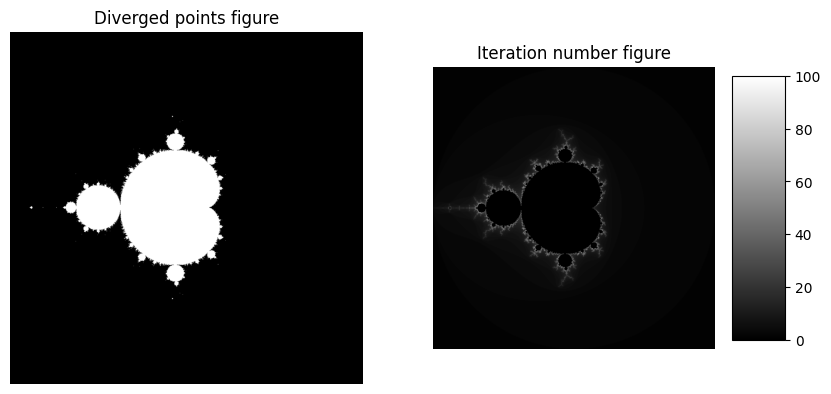
\includegraphics[width=\textwidth]{Plots/Q_1.png}
    \caption{The figure on the left shows the image with the diverged points in black and the non-diverged ones in white for the iteration done. While the figure on the right shows the iteration number based on the colour scale for each point. The iterations are based on the equation $z_{i+1} = z_i + c$ where the $c = x + iy$ and x and y are the x and y coordinates on the image.}
    \label{fig: Q1}
\end{figure}

\begin{figure}[hbt!]
    \centering
    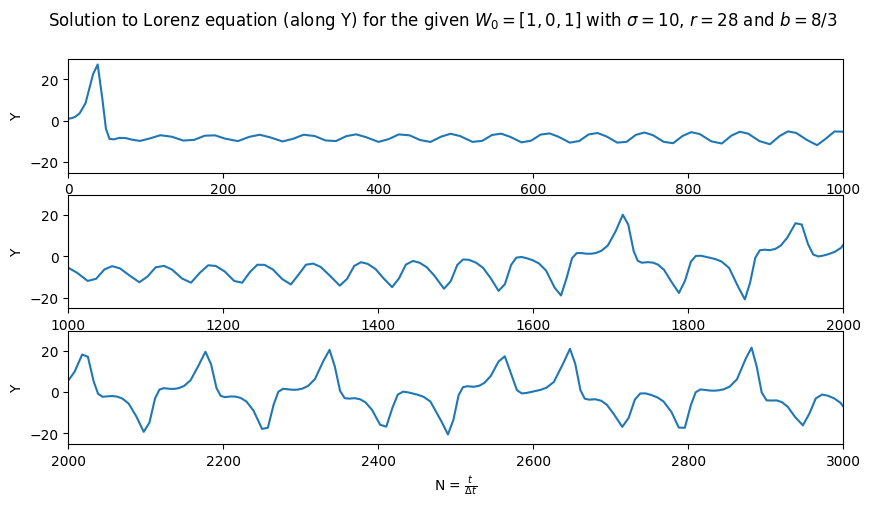
\includegraphics[width=\textwidth]{Plots/Q2_3.png}
    \caption{The figure shows the evolution of solution to the Lorenz equation for the initial condition [0, 1, 0] and parameters ($[\sigma, r, b] = [10, 28, 8/3]$) in Y direction for the first 30 seconds (or 3000 iterations). NOTE: TYPO in the title of the figure $W_0 = [0, 1, 0]$}
    \label{fig: Q2_3}
\end{figure}

\begin{figure}[hbt!]
    \centering
    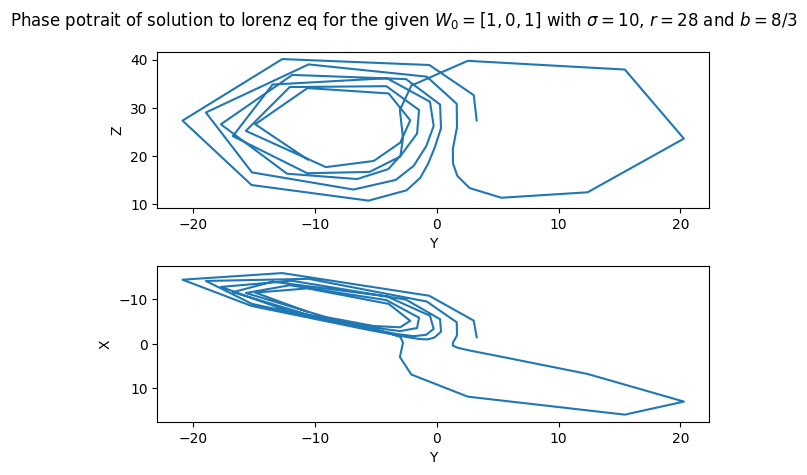
\includegraphics[width=\textwidth]{Plots/Q2_4.png}
    \caption{The figure shows the evolution of solution to the Lorenz equation for the initial condition [0, 1, 0] and parameters ($[\sigma, r, b] = [10, 28, 8/3]$) as phase portraits for the iterations 1400-1900. NOTE: TYPO in the title of the figure $W_0 = [0, 1, 0]$}
    \label{fig: Q2_4}
\end{figure}

\begin{figure}[hbt!]
    \centering
    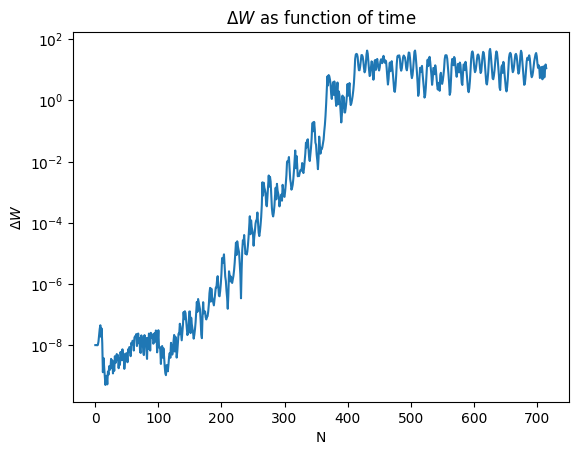
\includegraphics[width=\textwidth]{Plots/Q2_5.png}
    \caption{The figure shows the divergence in the two solutions to the Lorenz equation where the initial conditions for first solution are $W = [0, 1, 0]$ and for the second solution;$W = [0, 1 + 10^{-8}, 0]$  with parameters ($[\sigma, r, b] = [10, 28, 8/3]$).}
    \label{fig: Q2_5}
\end{figure}

\end{document}

%https://www.transcat.ca/media/pdf/U1250Series.pdf (multimeter handheld)

RL Filters
http://www.falstad.com/ci rcuit/e-filt-lopass-l.html
https://www.falstad.com/ circuit/e-filt-hipass-l.html